\documentclass{ucph-handout}
%\documentclass{article}
\usepackage[utf8]{inputenc}
\usepackage{listings}
\usepackage{xcolor}
\usepackage{amssymb}
\usepackage[danish]{babel}

%New colors defined below
\definecolor{codegreen}{rgb}{0,0.6,0}
\definecolor{codegray}{rgb}{0.5,0.5,0.5}
\definecolor{codepurple}{rgb}{0.58,0,0.82}
\definecolor{backcolour}{rgb}{0.95,0.95,0.92}

\lstdefinestyle{mystyle}{
  backgroundcolor=\color{backcolour},
  commentstyle=\color{codegreen},
  keywordstyle=\color{magenta},
  numberstyle=\tiny\color{codegray},
  stringstyle=\color{codepurple},
  basicstyle=\ttfamily\footnotesize,
  %breakatwhitespace=false,         
  %breaklines=true,                 
  captionpos=b,                    
  keepspaces=true,                 
  %numbers=left,                    
  %numbersep=5pt,                  
  showspaces=false,                
  showstringspaces=false,
  showtabs=false,                  
  tabsize=2
}

%"mystyle" code listing set
\lstset{style=mystyle}

\title{Machine Learning og huspriser}
\date{April 2020}
\renewcommand{\Author}{DIKU, 2020}
\newcommand{\Ark}{} % pt. ingen numre på arkene
\renewcommand{\Title}{\Ark Machine Learning og huspriser - Udforsk datasættet}

\newcommand{\inlinegraphics}[1]{\raisebox{-.3\height}{\includegraphics[height=1.5em]{#1}}}
\newcommand{\runbutton}{\inlinegraphics{images/run_button.png}}

\begin{document}
\begin{exercisebox}[adjusted title=Åbn ny Notebook]

Åbn hjemmesiden: \url{https://colab.research.google.com}, og opret en bruger eller login med din Google-konto.\\

Opret en ny notebook ved at trykke på knappen: 

\quad 
\includegraphics[height=2em]{images/colab_new_notebook_button}

Del din notebook med din gruppemakker, ved at trykke:

\quad
\includegraphics[height=3em]{images/colab_share_button.png}

\tcbsubtitle{Indlæs datasættet}
I den første celle indtaster I følgende, for at indlæse datasættet:
\begin{python}
import numpy as np
import matplotlib.pyplot as  plot
import housing_util

housing = housing_util.download_housing_data()
\end{python}

Tryk på knappen \runbutton\ for at køre koden og oprette en ny "kode celle".



%En Jupyter notebook er lavet af celler af tekst eller kode. Prøv at lave en celle ved at trykke på run knappen. Dette skulle gerne give os en ny celle under den gamle. Man kan også bruge genvejstasten. Man kan slette celler ved at trykke på dem med musen og derefter trykke \texttt{D} knappen 2 gange. \texttt{right-shift + Enter}

\tcbsubtitle{Inspicér datasættet}
Prøv nu at skriv følgende i den nye celle og tryk igen på \runbutton :
\begin{python}
housing.head()
\end{python}
I får nu vist en række for hver af de 5 første ejendomme i datasættet. 
Hvorfor er der i nogle tilfælde så mange rum?
\newline
\newline
For at se hvor mange ejendomme der er i alt, kan vi bruge \ttpy{len()} funktionen:
\begin{python}
len(housing)
\end{python}
Hver gang vi skal skrive noget nyt kode, skal vi lave en ny celle. Dette gør det nemmere at få et overblik over koden.
\tcbsubtitle{Celler i Google Colab}
En notebook består af en masse celler efter hinanden, enten indeholder de kode eller også indeholder de forklarende tekst.\newline

Menuen og værktøjslinjen kan du bruge til at arbejde med celler, fx:
\begin{itemize}
    \item Opret celle: Tryk på \inlinegraphics{images/new_cell} (eller \textit{Insert $\rightarrow$ Code cell} i menuen)
    \item Slet den valgte celle: Tryk på \textit{Edit $\rightarrow$ Delete Cells} i menuen
    %\item Skift type af celle: Brug dropdown-menuen \inlinegraphics{jupyter-toolbar.png} i toolbaren til at skifte om cellen indeholder kode (vælg \textrm{"Code"}) eller tekst (vælg \textrm{"Markdown"})
    \item Kør alle celler: Tryk på \inlinegraphics{images/runtime.png} og tryk Run all( \runbutton\ kører kun den valgte celle)
\end{itemize}

\end{exercisebox}
%%%%% Ark 1, side 2
\begin{exercisebox}[adjusted title=Udforsk datasættet]
Lad os prøve at forstå mere om datasættet. Prøv at beregn gennemsnittet af beboernes indkomst, ved at skrive følgende i en ny celle:
\begin{python}
gennemsnit = np.sum(housing["median_income"])/len(housing)
print(gennemsnit)
\end{python}

Hvad kan vi se her? Prøv selv at beregn gennemsnittet af nogle af de andre kolonner, for at blive endnu klogere på datasættet.
\tcbsubtitle{Histogrammer}
Udfra gennemsnit alene kan vi ikke sige så meget, hvis man gerne vil have et bedre overblik over dataet kan man bruge et histogram.\newline
\ \newline
Lav en ny celle og skriv:
\begin{python}
housing["median_income"].plot.hist(bins=10)
\end{python}
Hvad kan vi se på histogrammet? Prøv at ændre på \ttpy{bins}-argumentet:
\begin{python}
housing["median_income"].plot.hist(bins=50)
\end{python}
Hvad er forskellen? Udforsk de andre kolonner ved at lave flere histogrammer, for eksempel for \ttpy{total_rooms}, osv.
\end{exercisebox}

%\todo{Her er der plads til fx lidt mere om at bruge notebook-interfacet, fx hvordan de gemmer deres arbejde}
%\todo{En anden mulighed til hvad pladsen kan bruges på er mere detaljeret forklaring af hver kolonne i datasættet}

%%%%% Ark 2, side 1
\begin{exercisebox}[adjusted title=Vis data som landkort]
Vi har i datasættet længde- og breddegraderne for de forskellige huse. Med dem kan vi prøve at se om der er en forbindelse mellem forskellige datatyper og deres lokation. 
\vspace{-3mm}

Prøv at lave en ny celle og indtast følgende:
\begin{python}
housing.plot.scatter(x="longitude", y="latitude", figsize=(16,10))
\end{python}
Hvordan ser billedet ud? Prøv at udpege byer (sammenlign evt. med Google Maps)

\tcbsubtitle{Gør kortet nemmere at aflæse}
Hvis vi gerne vil gøre det nemmere at se, så kan vi lave prikkerne en smule gennemsigtige. Prøv at ændr i koden så der i stedet står\footnote{\texttt{alpha} er en værdi mellem $0.0$ og $1.0$, hvor $1.0$ er fuldt synlig og $0.0$ er helt gennemsigtig.}:
\begin{python}
housing.plot.scatter(x="longitude", y="latitude", figsize=(16,10), alpha=0.1)
\end{python}

Prøv også at ændre størrelsen af punkterne ved at sætte parameteret 's':
\begin{python}
housing.plot.scatter(x="longitude", y="latitude", figsize=(16,10),
                     alpha=0.1, s=50)
\end{python}
\vspace{-2mm}
\tcbsubtitle{Gør prikstørrelse afhængig af data}
At alle huse er samme størrelse giver ikke noget godt overblik. Prøv at sætte størrelsen `s` til at få sin værdi fra en parameter i datasættet, fx antal indbyggere:
\begin{python}
housing.plot.scatter(x="longitude",y="latitude", figsize=(16,10),
                     alpha=0.1, s=housing["population"])
\end{python}
Kan det kort fortælle os noget? En god data visualisering kommunikerer noget væsentlig information om dataet, kan vi aflæse noget fra kortet som det er nu?

\ \newline
Prøv at lave kortet med andre variabler, og se om I kan finde noget interessant at sige. F.eks. beboernes indkomst eller husenes alder. (Opret evt. nye celler)

\tcbsubtitle{Farveskala}
Vi kan plotte mere data ved at farve punkterne forskellige farver. Det kan gøres med argumenterne \ttpy{c} og \ttpy{colormap}. \footnote{Argumentet \ttpy{colormap} angiver farveskalaen, se alternativer til \ttpy{jet} inde på \url{https://matplotlib.org/3.1.1/gallery/color/colormap_reference.html}}
\begin{python}
housing.plot.scatter(x="longitude", y="latitude", figsize=(16,10),
                    alpha=0.4, s=housing["population"]/100,
                    c="median_house_value", 
                    colormap="jet")
\end{python}

\textbf{Opgaver:}
\vspace{-3mm}
\begin{itemize}
    \item Lav et kort af median indkomsten. Udfra dette kan man sige noget om forskellen mellem fordeling af median indkomst og huspriser?
    \item Overvej om I kan kombinere flere variabler. Hvad hvis vi fx vil se hvor mange de bor per rum, og altså ikke bare totalt antal beboere i ejendommen?
    \item Lav et kort over husenes alder. Kan man sige noget om forskellen mellem husenes alder og deres priser?
\end{itemize}
\vspace{-4mm}
\end{exercisebox}

%%%%% Ark 2, side 2
\begin{exercisebox}[adjusted title=At finde sammenhænge i data]
Prøv at indtaste følgende i en ny celle for at beregne en \textit{correlation matrix}:
\begin{python}
corr_matrix = housing.corr()
corr_matrix
\end{python}
Koefficienterne i matricen angiver for hvert par af variable, hvor meget den ene variabel stiger eller falder, når den anden variabel stiger. Jo tættere en koefficient er på 0, jo mindre sammenhæng er der mellem de to variabler.

\tcbsubtitle{Visualisere sammenhænge}
Der er forskellige måder at vise sammenhængene grafisk. En meget direkte måde er at plotte hele datasættet med de to variable man vil undersøge sat op mod hinanden:
\begin{python}
housing.plot.scatter(x="median_income", y="median_house_value", alpha=0.1)
\end{python}
Her har vi sat \ttpy{median_income} på x-aksen og \ttpy{median_house_value} på y-aksen. \newline

\vspace{-2mm}
\textbf{Opgaver:}
\vspace{-2mm}
\begin{itemize}
    \item Hvad siger plottet om forbindelsen mellem husenes pris og beboernes indkomst?
    \item Prøv at finde sammenhæng mellem andre variabler, f.eks. \ttpy{total_rooms} og \ttpy{median_value}
\end{itemize}

\end{exercisebox}
\begin{exercisebox}[adjusted title=Kombiner variabler]
Vi kan eksperimentere med nogle af variablerne, for at finde andre variabler. f.eks. kan vi beregne antal rum per husholdning via \ttpy{total_rooms} og \ttpy{households}.
\begin{python}
housing["rooms_per_household"] = housing["total_rooms"]/housing["households"]

\end{python}
Nu kan vi prøve at plotte vores nye variabel og se sammenhænge med huspriser\footnote{Ved at tilføje linjen \ttpy{ax.set_xlim(0, 20)} begrænser vi x-aksen til at gå fra 0 til 20, for ikke at se outliers (prøv evt. uden denne linje)}:
\begin{python}
ax=housing.plot.scatter(x="rooms_per_household", y="median_house_value", 
                        alpha=0.1)
ax.set_xlim(0, 20)
\end{python}

Hvilken form for sammenhæng kan vi aflæse af plottet?

\tcbsubtitle{Flere variabler}
Prøv også at beregn antal værelser per husholdning, eller antal beboere per husholdning:
\begin{python}
housing["bedrooms_per_household"] = housing["total_bedrooms"]/housing["households"]
housing["population_per_household"] = housing["population"]/housing["households"]
\end{python}

\textbf{Opgaver:}
\vspace{-2mm}
\begin{itemize}
    \item Plot sammenhænge mellem de nye variabler og \ttpy{median_income}
    \item Hvilken sammenhæng kan vi se mellem, hvor mange der lever sammen, og hvor rige folk er?
\end{itemize}

\end{exercisebox}

%%%%% Ark 3, side 1
\newpage
\renewcommand{\Title}{\Ark Machine Learning og huspriser - Klargøring}%
\begin{exercisebox}[adjusted title=Klargøring]
Inden vi går i gang med machine learning-delen, så bør I tjekke om I stadig har adgang til datasættet vi indlæste i går.\newline

Skriv \ttpy{housing.head()} i en celle og kør cellen: \\
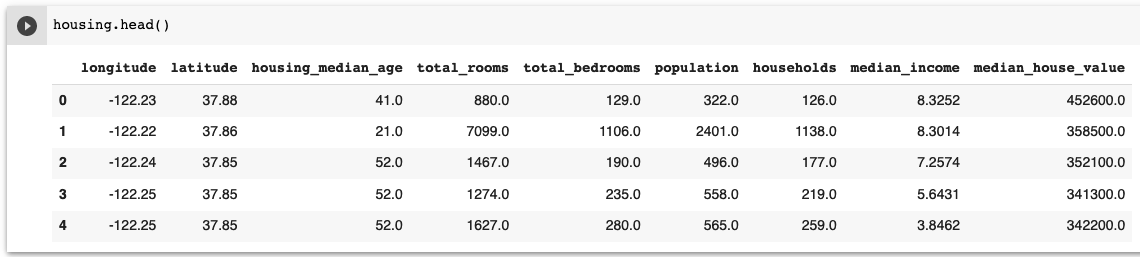
\includegraphics[width=\textwidth]{images/dataset_head}

Hvis ikke det lykkes for jer, så gå tilbage til det vi startede med i går og gentag det for at indlæse datasættet igen.
\end{exercisebox}


%\begin{itemize}
%    \item 
%    \item 
% \end{itemize}


\begin{exercisebox}[adjusted title=Opdeling i labels og features]
Målet er jo at vi skal lave en machine learning model der kan gætte huspriser (\ttpy{"median_house_value"}), ud fra de andre værdier (\ttpy{"total_rooms"}, \ttpy{"latitude"}, osv.)\\ % \ttpy{"bedrooms_per_household"},  osv.).\\

For at kunne adskille de to ting, kalder man det første for \textit{labels} (det der skal gættes) og det andet for \textit{features} (de værdier gættet baserer sig på). I kode kan vi opdele de to ting på følgende måde:
\begin{python}
labels = housing["median_house_value"]
features = housing.drop("median_house_value", axis = 1)
\end{python}


Den første linje, fjerner \ttpy{"median_house_value"} kolonnen fra \ttpy{"housing"}, den anden linje giver os \ttpy{"median_house_value"} alene, uden alt det andet.\\

Prøv at vise de to på skærmen, og se hvordan de ser ud (brug evt. \ttpy{.head()})

\tcbsubtitle{Skalering}
Vi har også et andet problem. Vores værdier er meget forskellige i størrelse, fx er \ttpy{total_rooms} i et eksempel helt oppe på 7099.0, mens \ttpy{median_income} højest bliver 15. Det betyder at de høje værdier, vil få større indflydelse end de lave værdier, så vores machine learning model vil blive meget mere påvirket af antallet af værelser på fx $7099$ værelser, end af median indkomsten (som fx er $8.3014$).\\

Vi kan undgå det ved at skalere alle tallene, så ingen har mere indflydelse end andre:
\begin{python}
from sklearn.preprocessing import StandardScaler
scaler = StandardScaler()
scaler.fit(features)
scaled_features = scaler.transform(features)
\end{python}

Prøv at se hvordan jeres \ttpy{features} ser ud nu.
\end{exercisebox}

%\newpage

\begin{exercisebox}[adjusted title=Opdeling af datasættet]
Vi mangler en sidste ting inden vi kan træne vores machine learning model. For at kunne afprøve hvor godt vores træning går, skal vi have opdelt datasættet i en del til træning og en anden del som kan bruge til afprøvning:
\begin{itemize}
    \item et \textit{træningssæt} til at træne vores model
    \item og et \textit{testsæt} til at afprøve vores model
\end{itemize}
I vores tilfælde vil vi gerne have $80\%$ data til træning af vores model, og de resterende 20\% til at afprøvning af vores model. \\

For at gøre det regner vi først ud hvor datasættet skal opdeles (efter $20\%$)
\begin{python}
split = int(len(housing)*0.2)
\end{python}

Så kan vi først opdele vores features, så de første 20\% bliver til testsæt og de resterende til træningssæt:
\begin{python}
test_features = scaled_features[:split]
training_features = scaled_features[split:]
\end{python}

Gør det samme for labels:
\begin{python}
test_labels = labels[:split]
training_labels = labels[split:]
\end{python}

Notationen \ttpy{scaled_features[:split]} betyder "tag alt data \textit{hen til} splitpunktet". Omvendt betyder notationen \ttpy{scaled_data[split:]} at vi vil have alt data \textit{fra} splitpunktet og hen til slutningen.
\end{exercisebox}

\newpage
\renewcommand{\Title}{\Ark Machine Learning - træning og afprøvning af modeller}%

\begin{exercisebox}[adjusted title=Lineær regression som Machine Learning model]
Når vi har fået forberedt vores datasæt, er vi klar til at træne machine learning modellen. Vi vil starte med en lineær regressions model. Den oprettes sådan:
\begin{python}
from sklearn.linear_model import LinearRegression
lin_model = LinearRegression()
\end{python}

Efter vi har oprettet modellen, kan vi træne den ved at kalde \ttpy{.fit()} funktionen med vores træningsdata:
\begin{python}
lin_model.fit(training_features, training_labels)
\end{python}

Nu er vores model \ttpy{lin_model} trænet, og klar til at kunne forudsige huspriser

\tcbsubtitle{Afprøvning af modellen}

Lad os starte med at afprøve machine learning modellen på det første hus i testsættet:
\begin{python}
test_house = test_features[0]
\end{python}

For at forudse hvilken pris det hus skal have, kan vi kalde \ttpy{predict()} på vores model:
\begin{python}
lin_model.predict([test_house])
\end{python}


Hvor langt er forudsigelsen fra den rigtige pris på huset? Hvor tæt ser den ud til at ramme, hvis I prøver med nogle af de andre huse?

\tcbsubtitle{Kan vi måle hvor god vores model er?}
For at vurdere hvor godt modellen fungerer helt generelt, kan vi prøve den af på alle værdierne i vores testsæt. \newline

Først forudsiger vi priserne for alle husene i testsættet:

\begin{python}
predictions = lin_model.predict(test_features)
\end{python}

Nu har vi en liste af forudsigelser, som vi kan sammenligne med værdierne i \ttpy{test_labels}, for at se hvor meget de afviger.\newline

Til at gøre det bruger man en speciel målestok der hedder \textit{root mean squared error}. Det kan man beregne sådan her:

\begin{python}
from sklearn.metrics import mean_squared_error
mse = mean_squared_error(test_labels, predictions)
rmse = np.sqrt(mse)
\end{python}

Den første linje importerer en funktion, \ttpy{mean_squared_error}, som vi bruger i den næste linje. I den sidste linje tager vi bare kvadratroden (\texttt{sqrt} = square root) af resultatet fra linjen før.

\end{exercisebox}
\begin{exercisebox}[adjusted title=Sammenlign med Decision tree regræssionsmodel]
Lineær regression kender I måske allerede fra jeres matematik timer, en mere avanceret metode baserer sig på \textit{beslutningstræer} (eng. decision trees).\newline

Kodemæssigt er den eneste forskel fra lineær regression  at vi opretter vores ikke-trænede model via de her to linjer:
\begin{python}
from sklearn.tree import DecisionTreeRegressor
tree_model = DecisionTreeRegressor()
\end{python}

Derefter kan I prøve at træne \ttpy{tree_model} modellen og lave forudsigelser, på helt samme måde som I gjorde med lineær regression. Bare erstat \ttpy{lin_model} med \ttpy{tree_model} alle steder, og se hvor meget værre/bedre decision trees er til at lave forudsigelser på det her problem.\newline

Hvilken af de to modeller klarer sig bedst?\newline
Prøv evt. at køre koden der laver decision tree modellen flere gange.


%\begin{python}
%from sklearn.tree import DecisionTreeRegressor
%tree_model = DecisionTreeRegressor()
%tree_model.fit(training_data, training_labels)
%tree_result = tree_model.predict(test_data);
%tree_mse = mean_squared_error(test_labels, tree_result)
%tree_rmse = np.sqrt(tree_mse);

%print("DecisionTree: " + str(decision_rmse))
%\end{python}
%Hvad sker der hvis du kører koden igen?\newline
%Hvilken en af de 2 modeller klare sig bedst? \newline

\end{exercisebox}
\begin{exercisebox}[adjusted title=Random forest - endnu en machine learning model]

Lad os prøve en tredje model, kaldet \textit{Random forest}, der består af mange forskellige decision trees, og når der forudsiges, tage gennemsnittet af de mange decision tree modellers forudsigelser.

Kodemæssigt, oprettes modellen sådan:
\begin{python}
from sklearn.ensemble import RandomForestRegressor
forest_model = RandomForestRegressor(n_estimators=10)
\end{python}

Her har vi angivet at der skal bruges 10 decision trees. Prøv at træn modellen på samme måde som med de tidligere modeller.\\

Hvor meget bedre er random forest, end en model med et enkelt decision tree? Prøv evt. at sætte antallet af decision trees op til 100 eller 200.\\


\end{exercisebox}

\end{document}
